% !TeX root = RJwrapper.tex
\title{Reproducible Summary Tables with the \pkg{gtsummary} Package}
\author{by Daniel D. Sjoberg, Karissa Whiting, Michael Curry}

\maketitle

% TO DO
% - add/remove the page breaks as needed (when it's ready to be submitted)

\abstract{
The \pkg{gtsummary} package provides an elegant and flexible way to create publication-ready summary tables in R.
A critical part of the work of statisticians, data scientists, and analysts is summarizing data sets and regression models in R and publishing or sharing polished summary tables.
The \pkg{gtsummary} package was created to streamline these everyday analysis tasks by allowing users to easily create reproducible summaries of data sets, regression models, survey data, and survival data with a simple interface and very little code.
The package follows a tidy framework, making it easy to integrate in standard data workflows, and offers many table customization features through function arguments, helper functions, and custom themes.
}

\section{Introduction}

Table summaries are a fundamental tool in an analyst's toolbox that help us understand and communicate patterns in our data.
The ability to easily create and export polished and reproducible tables is essential.
The \CRANpkg{gtsummary} \citep{gtsummary} package provides an elegant and flexible framework to create publication-ready analytical and summary tables in R.
This package works to close the gap between a reproducible RMarkdown report and the final report.
Specifically, \pkg{gtsummary} allows the us to fully customize and format summary tables with code, eliminating the need to modify any tables by hand after the table has been exported.
Removing the need to modify tables after the table has been created eliminates an error-prone step in our workflow, and increases the reproducibility of our analyses and reports. 

Using \pkg{gtsummary}, analysts can easily summarize data frames, present and compare descriptive statistics between groups, summarize regression models, and report statistics inline in RMarkdown reports. 
After identifying these basic structures of most tables presented in medical literature (and other fields), we created \pkg{gtsummary} to ease creation of fully-formatted, ready to publish tables.

Additionally, \pkg{gtsummary} leverages other analysis and tidying R packages to create a complete analysis and reporting framework.
For example, we take advantage of the existing \CRANpkg{broom} tidiers to prepare regression results for \code{tbl\_regression()} and use \CRANpkg{gt} \citep{gt} to print \pkg{gtsummary} tables to various output formats (e.g. HTML, PDF, Word, or RTF).
Furthermore, \pkg{gtsummary} functions are designed to work within a "tidy" framework, utilizing the \CRANpkg{magrittr} pipe operator and \CRANpkg{tidyselect} \citep{tidyselect} functions used throughout the \CRANpkg{tidyverse} \citep{tidyverse}.

While other R packages are available to clean and present summary statistics and regression results in statistical reports, \pkg{gtsummary} is unique in that it is a one-stop-shop for most types of statistical tables and offers diverse features to customize content of tables to a high degree. It also includes the ability to report statistics from the tables inline in an RMarkdown report.
For example other summary statistics packages such as \CRANpkg{skimr}, \CRANpkg{summarytools}, and \CRANpkg{tableone} provide detailed descriptive statistics, but at least one major advantage of \CRANpkg{gtsummary} is the ability to also provide these same descriptive statistics that are publication ready in a scientific journal with little or no additional formatting.
Additionally \CRANpkg{gtsummary} has specific internal algorithms to identify variable data types so the user does not have to specify if a variable should be displayed with categorical or continuous summaries, unlike  \CRANpkg{tableone}.
However, it is possible to override \CRANpkg{gtsummary} variable selection defaults if the users chooses too. 
%For example with \CRANpkg{finalfit}, you have to manually specify a printing engine for the table to render.
%Furthermore, \CRANpkg{tableone} reports on general descriptive statistics, but it is lacking in its ability to produce tables for regression modeling strategies in R. 

Along with descriptive summaries, \pkg{gtsummary} summarises statistical models, survey data, and builds cross tabulations. 
After data are summarized in a table, \pkg{gtsummary} allows users to combine tables, either side-by-side (with \code{tbl\_merge()}) , or on top of each other (with \code{tbl\_stack()}). 
This table merging and stacking allows us to easily synthesize and compare output from several tables and share information in a compact format.   

\section{Data Summaries}

To showcase \pkg{gtsummary} functions, we will use a simulated clinical trial data set containing baseline characteristics of 200 patients who received Drug A or Drug B, as well as the outcomes of tumor response and death.
Each variable in the data frame has been assigned an attribute label with the \pkg{labelled} package \citep{labelled}, e.g. \code{trial \%>\% set\_variable\_labels(age = "Age")} that will be shown in the summary tables. 
These labels are displayed in the \pkg{gtsummary} tables by default, and had labels not been assigned the variable name would have been shown.

% adding table describing trial dataset
\captionsetup[table]{labelformat=empty,skip=1pt}
\begin{longtable}{llll}
\toprule
colname & label & class & values \\ 
\midrule
\texttt{trt} & Chemotherapy Treatment & character & \texttt{Drug A}, \texttt{Drug B} \\ 
\texttt{age} & Age & numeric & \texttt{6}, \texttt{9}, \texttt{10}, \texttt{17}, ... \\ 
\texttt{marker} & Marker Level (ng/mL) & numeric & \texttt{0.003}, \texttt{0.005}, \texttt{0.013}, \texttt{0.015}, ... \\ 
\texttt{stage} & T Stage & factor & \texttt{T1}, \texttt{T2}, \texttt{T3}, \texttt{T4} \\ 
\texttt{grade} & Grade & factor & \texttt{I}, \texttt{II}, \texttt{III} \\ 
\texttt{response} & Tumor Response & integer & \texttt{0}, \texttt{1} \\ 
\texttt{death} & Patient Died & integer & \texttt{0}, \texttt{1} \\ 
\texttt{ttdeath} & Months to Death/Censor & numeric & \texttt{3.53}, \texttt{5.33}, \texttt{6.32}, \texttt{7.27}, ... \\ 
\bottomrule\caption{\label{tab:caption}Table 1. Example data frame, \texttt{trial}}\\

\end{longtable}



\subsection{\texorpdfstring{\code{tbl\_summary()}}{tbl\_summary()}}

The default output from \code{tbl\_summary()} is meant to be publication ready.
The \code{tbl\_summary()} function can take, at minimum, a data frame as the only input, and returns descriptive statistics for each column in the data frame.
This is often the first table of clinical manuscripts and describes characteristics of the study cohort.
A simple example is shown below.
Notably, by specifying the \code{by=} argument, you can stratify the summary table. 
In the example below, we have split the table by the treatment a patient received. 

% code for basic tbl_summary()
% \newpage
\begin{example}
trial %>%
  select(age, grade, response, trt) %>%
  tbl_summary(by = trt)
\end{example}
\begin{figure}[h!]
  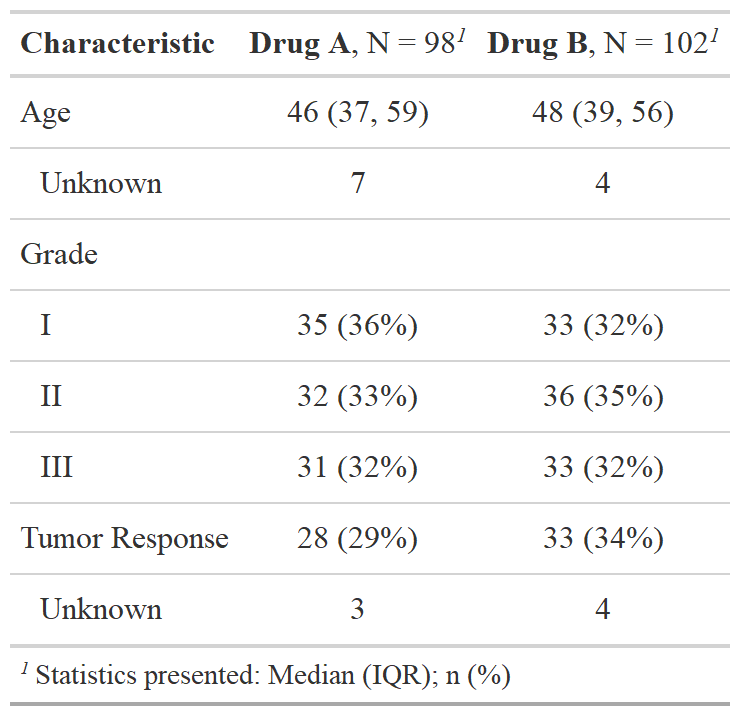
\includegraphics[scale=0.49]{summary_basic.png}
  \centering
\end{figure}

The function is highly customizable, and it is initiated with sensible default settings.
Specifically, \code{tbl\_summary} detects variable types of input data and calculates descriptive statistics accordingly.
For example, variables coded as \code{0/1}, \code{TRUE/FALSE}, and \code{Yes/No} are presented dichotomously.
Additionally, \code{NA} values are recognized as missing and listed as unknown, and if a data set is labelled, the label attributes are automatically utilized. 

Default settings may be customized using the \code{tbl\_summary()} function arguments.

% code for tbl_summary() with arguments
\captionsetup[table]{labelformat=empty,skip=1pt}
\begin{longtable}{ll}
\toprule
Argument & Description \\ 
\midrule
\texttt{label=} & specify the variable labels printed in table \\ 
\texttt{type=} & specify the variable type (e.g., continuous, categorical, etc.) \\ 
\texttt{statistic=} & change the summary statistics presented \\ 
\texttt{digits=} & number of digits the summary statistics will be rounded to \\ 
\texttt{missing=} & whether to display a row with the number of missing observations \\ 
\texttt{missing\_text=} & text label for the missing number row \\ 
\texttt{sort=} & change the sorting of categorical levels by frequency \\ 
\texttt{percent=} & print column, row, or cell percentages \\ 
\texttt{include=} & list of variables to include in summary table \\ 
\caption{\label{tab:}\texttt{tbl\_summary()} function arguments}\\
\bottomrule
\end{longtable}



For continuous variables, tables display one row of statistics per variable by default.
This can be customized, and in the example below the age variable is cast to \code{"continuous2"} type, meaning the continuous summary statistics will appear on two or more rows in the table. 
This allows the number of non-missing observations and the mean to be displayed on separate lines.

In the example below, the \code{"age"} variable's label is updated to \code{"Patient Age"}.
Default summary statistics for both continuous and categorical variables are updated using the \code{statistic=} argument. 
\pkg{gtsummary} uses \CRANpkg{glue} \citep{glue} syntax construct the statistics displayed in the table.
Function names appearing in curly brackets will be replaced by the evaluated value.
The \code{digits=} argument is used to increase the number of decimal places to which the statistics are rounded, and the missing row is omitted with \code{missing = "no"}.

% \newpage
\begin{example}
trial %>%
  select(age, grade, response, trt) %>%
  tbl_summary(
    by = trt,
    type = age ~ "continuous2",
    label = age ~ "Patient Age",
    statistic = list(age ~ c("{N_nonmiss}", "{mean} ({sd})"),
                     c(grade, response) ~ "{n} / {N} ({p}%)"),
    digits = c(grade, response) ~ c(0, 0, 1),
    missing = "no"
  )
\end{example}
\begin{figure}[h!]
  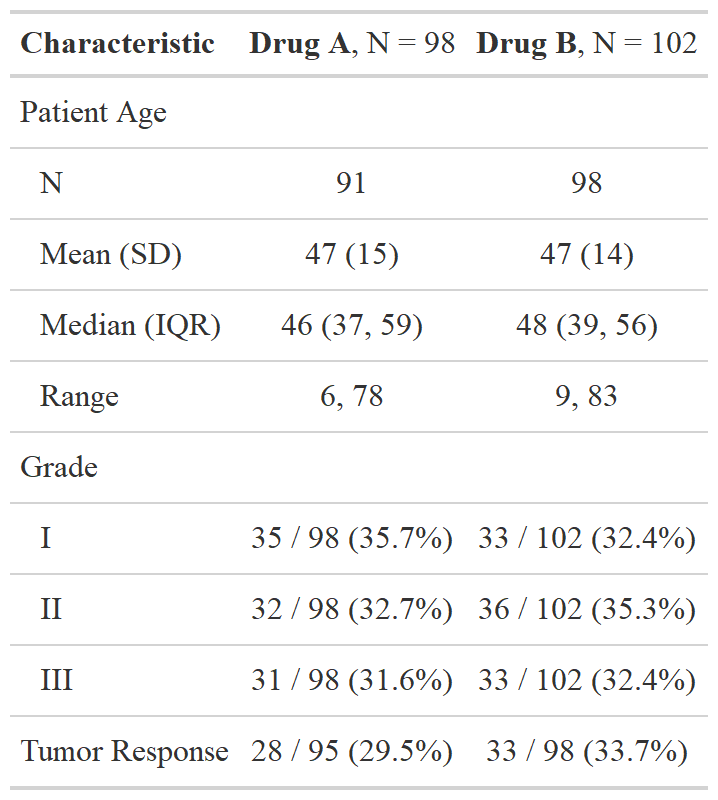
\includegraphics[scale=0.49]{summary_plus.png}
  \centering
\end{figure}

\textbf{A note about notation:}
Throughout the \pkg{gtsummary} package, you'll find function arguments that accept a list of formulas (or a single formula) as the input.
In the example above, the label for the age variable was updated using \code{label = age $\sim$ "Patient Age"}---equivalently, \code{label = list(age $\sim$ "Patient Age")}.
To select groups of variables, utilize the select helpers from the \pkg{tidyselect} and \pkg{gtsummary}.
The \code{all\_continuous()} selector is a convenient way to select all continuous variables.
In the example above it could have been used to change the summary statistics for all continuous variables---\code{all\_continuous() $\sim$ c("\{N\_nonmiss\}", "\{mean\} (\{sd\})")}. 
Similarly, users may utilize \code{all\_categorical()} (from \pkg{gtsummary}), or any of the \pkg{tidyselect} helpers used throughout the \pkg{tidyverse} package, such as \code{starts\_with()}, \code{contains()}, etc.

In addition to summary statistics, the \pkg{gtsummary} package has several functions to add additional information or statistics to \code{tbl\_summary()} tables.

% code for tbl_summary() with arguments
\captionsetup[table]{labelformat=empty,skip=1pt}
\begin{longtable}{ll}
\toprule
Function & Description \\ 
\midrule
\texttt{add\_p()} & add \emph{p}-values to the output comparing values across groups \\ 
\texttt{add\_overall()} & add a column with overall summary statistics \\ 
\texttt{add\_n()} & add a column with N (or N missing) for each variable \\ 
\texttt{add\_difference()} & add column for difference between two group, confidence interval, and \emph{p}-value \\ 
\texttt{add\_stat\_label()} & add label for the summary statistics shown in each row \\ 
\texttt{add\_stat()} & generic function to add a column with user-defined values \\ 
\texttt{add\_q()} & add a column of \emph{q}-values to control for multiple comparisons \\ 
\bottomrule\caption{\label{tab:caption}Table 3. \texttt{tbl\_summary()} functions to add information}\\

\end{longtable}



In the example below the number of non-missing observations is reported for each variable, as well as a p-value comparing the values between the treatment.
Default statistical tests are chosen based on data type, and the statistical test performed can be customized in the \code{add\_p()} function.
P-value formatting can be adjusted using the \code{pvalue\_fun=} argument which accepts both a proper function, as well the formula shortcut notation used throughout the \pkg{tidyverse} packages.

\newpage
\begin{example}
trial %>%
  select(age, grade, response, trt) %>%
  tbl_summary(by = trt, missing = "no") %>%
  add_n() %>%
  add_p(test = all_continuous() ~ "t.test",
        pvalue_fun = ~style_pvalue(., digits = 2))

\end{example}
\begin{figure}[h!]
  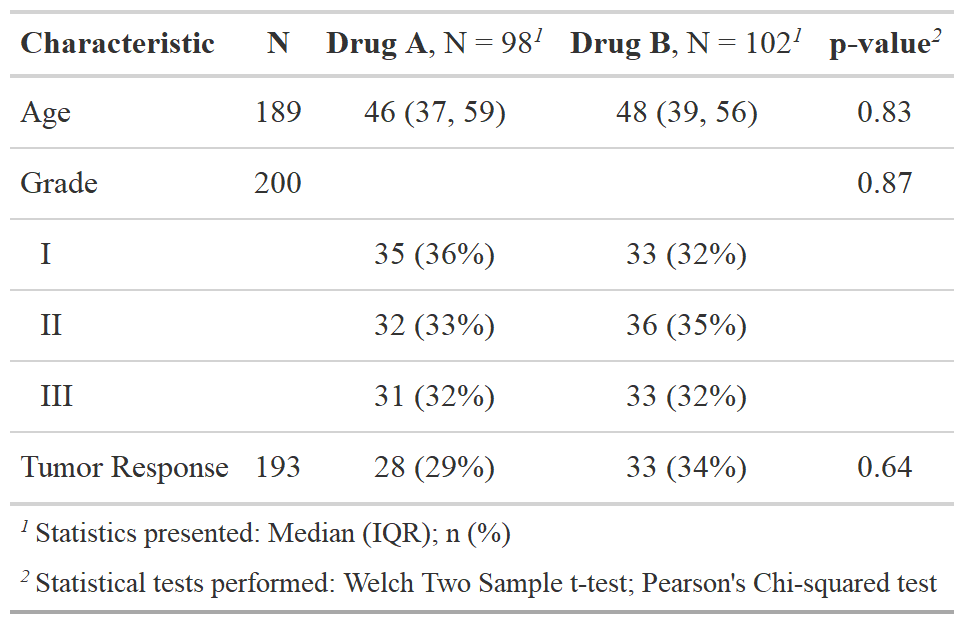
\includegraphics[scale=0.49]{summary_plus_plus.png}
  \centering
\end{figure}

\subsection{\texorpdfstring{\code{tbl\_svysummary()}}{tbl\_svysummary()}}

The \code{tbl\_svysummary()} function is analagous to \code{tbl\_summary()} except an \CRANpkg{survey} \citep{survey} object is supplied rather than a data frame.
The summary statistics presented take into account the survey weights, as do any p-values presented.

% \newpage
\begin{example}
# convert trial data frame to survey object
svy_trial <- survey::svydesign(data = trial, ids = ~ 1, weights = ~ 1)

tbl_svysummary_1 <-
  svy_trial %>%
  tbl_svysummary(by = trt, include = c(trt, age, grade)) %>%
  add_p()
\end{example}
\begin{figure}[h!]
  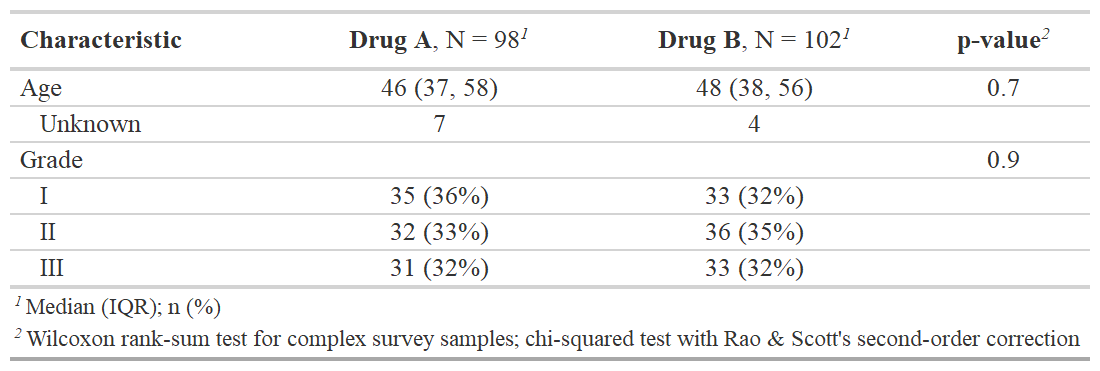
\includegraphics[scale=0.49]{svysummary.png}
  \centering
\end{figure}

\subsection{\texorpdfstring{\code{tbl\_cross()}}{tbl\_cross()}}

The \code{tbl\_cross()} function is a wrapper for \code{tbl\_summary()} and creates a simple, publication-ready cross tabulation.

\newpage
\begin{example}
trial %>%
  tbl_cross(row = stage, col = trt, percent = "cell") %>%
  add_p(source_note = TRUE)
\end{example}
\begin{figure}[h!]
  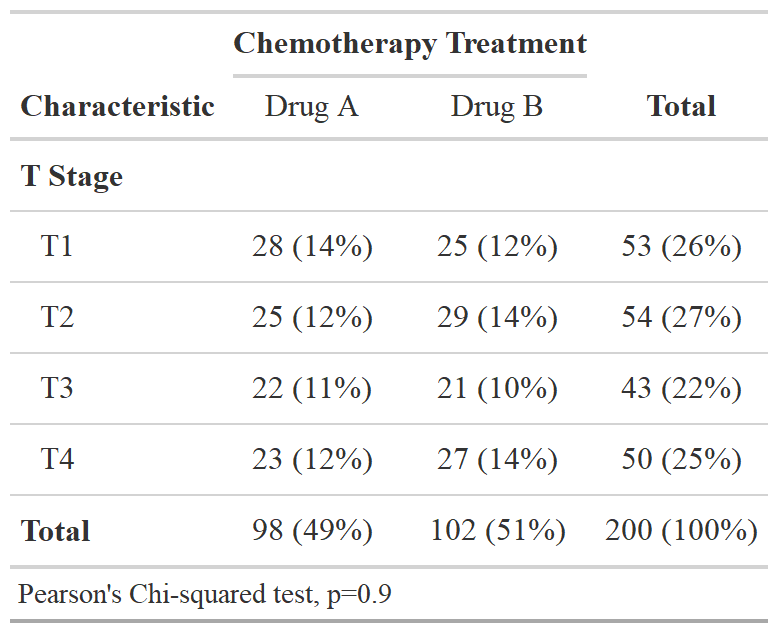
\includegraphics[scale=0.49]{cross.png}
  \centering
\end{figure}

\subsection{\texorpdfstring{\code{tbl\_survfit()}}{tbl\_survfit()}}

The \code{tbl\_survfit()} function parses and tabulates \code{survival::survfit()} objects presenting survival percentile estimates and survival probabilities at specified times. 

% \newpage
\begin{example}
library(survival)

list(survfit(Surv(ttdeath, death) ~ trt, trial),
     survfit(Surv(ttdeath, death) ~ grade, trial)) %>%
  tbl_survfit(times = c(12, 24),
              label_header = "**{time} Month**") %>%
  add_p()
\end{example}

\begin{figure}[h!]
  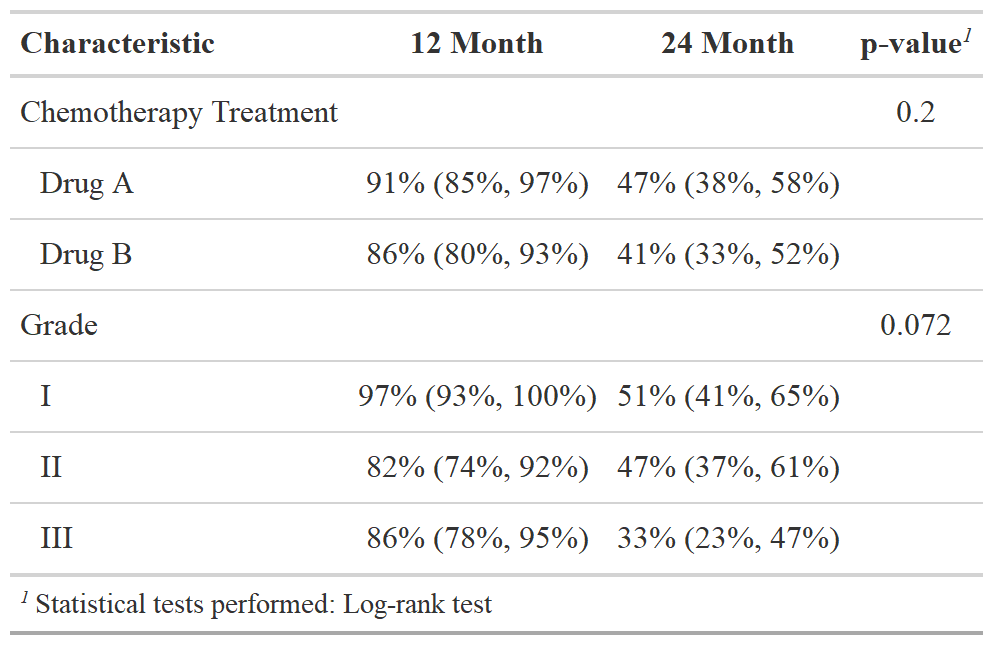
\includegraphics[scale=0.49]{survfit.png}
  \centering
\end{figure}

\subsection{Customization}

The \pkg{gtsummary} package includes functions specifically made to modify and format the summary tables.
These functions work with any table constructed with \pkg{gtsummary}.
Most common uses are changing the column headers and footnotes, or modifying the look of tables through bolding and italicization. 

% adding table describing fns for customization
\captionsetup[table]{labelformat=empty,skip=1pt}
\begin{longtable}{ll}
\caption{\label{tab:} Functions to style and modify gtsummary tables}\\
\toprule
Function & Description \\ 
\midrule
\texttt{modify\_header()} & update column headers \\ 
\texttt{modify\_footnote()} & update column footnote \\ 
\texttt{modify\_spanning\_header()} & update spanning headers \\ 
\texttt{modify\_caption()} & update table caption/title \\ 
\texttt{bold\_labels()} & bold variable labels \\ 
\texttt{bold\_levels()} & bold variable levels \\ 
\texttt{italicize\_labels()} & italicize variable labels \\ 
\texttt{italicize\_levels()} & italicize variable levels \\ 
\texttt{bold\_p()} & bold significant p-values \\ 
\bottomrule
\end{longtable}



The \pkg{gtsummary} package utilizes the \pkg{gt} package to print the summary tables.
The \pkg{gt} package exports approximately one hundred functions to customize and style tables.
When you need to add additional details or styling not available within \pkg{gtsummary}, use the \code{as\_gt()} function to convert the \pkg{gtsummary} object to gt and continue customization.

The example below includes customization using both \pkg{gtsummary} and \pkg{gt} functions.
The \pkg{gtsummary} functions are utilized to bold p-values below a threshold, bold the variable labels,  update the column header, and add a spanning header.
Additional \pkg{gt} customization was utilized to add table captions and source notes.

% \newpage
\begin{example}
trial %>%
  select(age, grade, trt) %>%
  tbl_summary(by = trt, missing = "no") %>%
  add_overall() %>%
  add_p() %>%
  add_q() %>%
  add_stat_label() %>%
  bold_p(t = 0.10) %>%
  bold_labels() %>%
  modify_header(label ~ "**Variable**") %>% 
  modify_spanning_header(c(stat_1, stat_2) ~ "**Treatment Received**") %>%
  as_gt() %>%
  gt::tab_header(
    title = gt::md("**Table 1. Patient Characteristics**"),
    subtitle = gt::md("_Highly Confidential_")
  ) %>%
  gt::tab_source_note("Data updated June 26, 2015")
\end{example}
\begin{widefigure}[h!]
  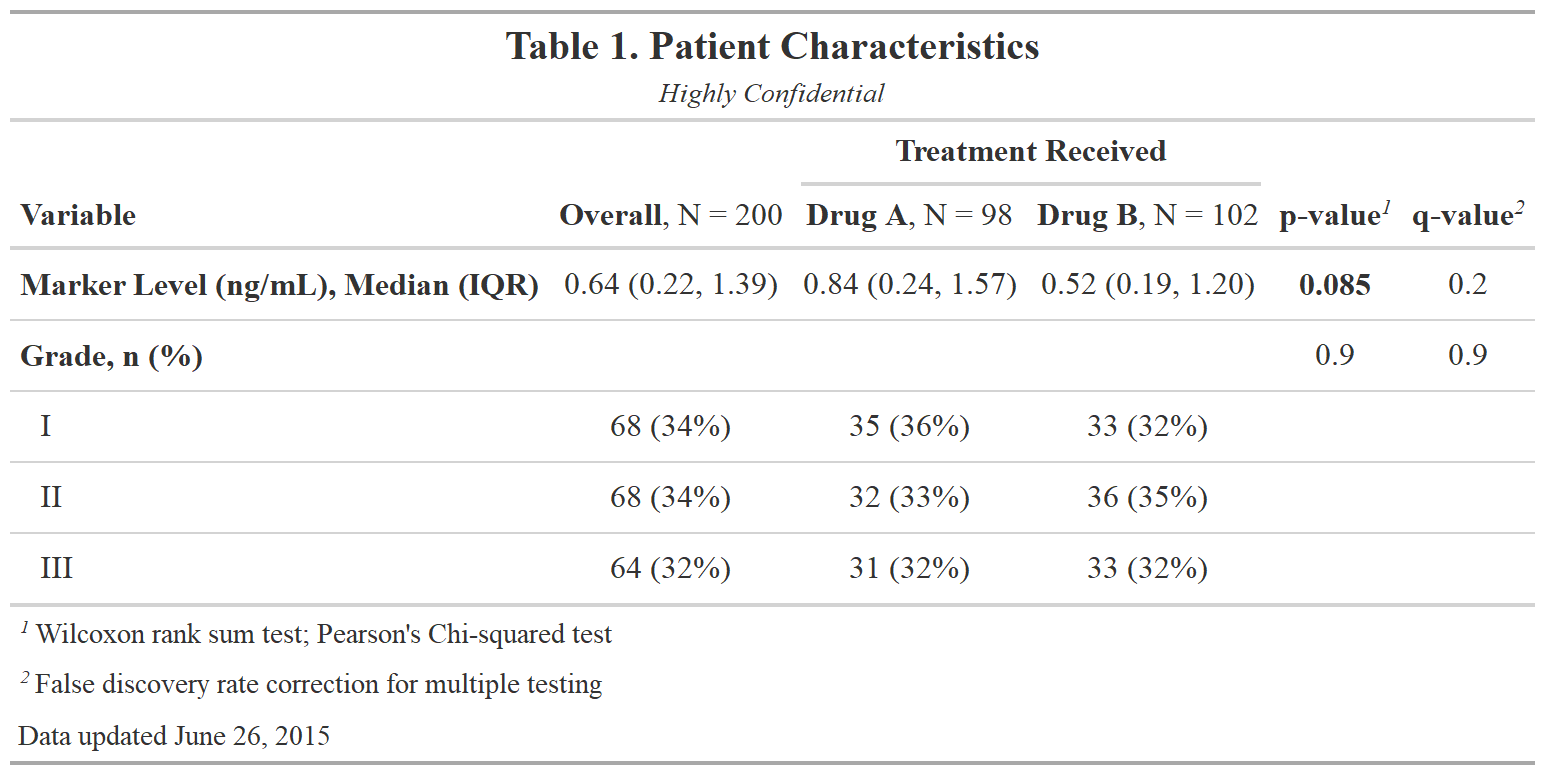
\includegraphics[scale=0.49]{custom.png}
  \centering
\end{widefigure}

\section{Model Summaries}

Regression modelling is one of the most common tools of medical research.
The \pkg{gtsummary} package has two functions to help analysts prepare tabular summaries of regression models: \code{tbl\_regression()} and \code{tbl\_uvregression()}.

\subsection{\texorpdfstring{\code{tbl\_regression()}}{tbl\_regression()}}

The \code{tbl\_regression()} function takes a regression model object in R and returns a formatted table of regression model results. 
Like \code{tbl\_summary()}, \code{tbl\_regression()} creates highly customizable analytic tables with sensible defaults.
Common regression models, such as logistic regression and Cox proportional hazards regression, are automatically identified and the tables headers are pre-filled with appropriate column headers (i.e. Odds Ratio and Hazard Ratio).

In the example below, the logistic regression model is summarized with \code{tbl\_regression()}.
Note that a reference row for Grade I has been added, and the variable labels have been carried through into the table.
Using \code{exponentiate = TRUE}  we exponentiate the regression coefficients, yielding the odds ratios.
The helper function \code{add\_global\_p()} was used to replace the p-values for each term with the global p-value for grade.

% \newpage
\begin{example}
glm(response ~ age + grade, trial, family = binomial) %>%
  tbl_regression(exponentiate = TRUE) %>%
  add_global_p()
\end{example}

\begin{figure}[h!]
  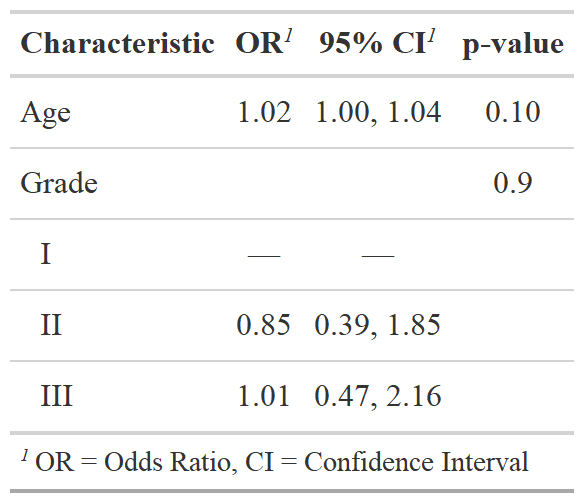
\includegraphics[scale=0.49]{regression.png}
  \centering
\end{figure}

The \code{tbl\_regression()} function leverages the huge effort behind the \pkg{broom} package's \code{tidy()} function to perform the initial formatting of the regression object \citep{broom}.
Because \code{tbl\_regression()} utilizes \code{broom::tidy()}, there are many model types that are supported out of the box, such as \code{lm()}, \code{glm()}, \code{lme4::lmer()}, \code{lme4::glmer()}, \code{geepack::geeglm()}, \code{survival::coxph()}, \code{survival::survreg()}, \code{survival::clogit()}, \code{nnet::multinom()}, \code{rstanarm::stan\_glm()}, and models built with the mice package[add ref]and more. The \pkg{gtsummary} package also contains built-in tidying functions to report standardized coefficients and bootstrapped confidence intervals.
A custom tidier may be specified as well, which is helpful when you need to present non-standard modifications to your model results such as Wald confidence intervals, or results with modified variance-covariance regression coefficients.

\subsection{\texorpdfstring{\code{tbl\_uvregression()}}{tbl\_uvregression()}}

The \code{tbl\_uvregression()} function is a wrapper for \code{tbl\_regression()} that is useful when you need a series of univariate regression models.
The user passes a data frame to \code{tbl\_uvregression()}, indicates what the outcome is, what regression model to run, and the function will return a formatted table of stacked univariate regression models.

\begin{example}
trial %>%
  select(response, age, grade) %>%
  tbl_uvregression(
    y = response, 
    method = glm,
    method.args = list(family = binomial),
    exponentiate = TRUE,
    pvalue_fun = ~style_pvalue(., digits = 2)
  ) %>%
  add_nevent() %>%
  add_global_p()
\end{example}
\newpage
\begin{figure}[h!]
  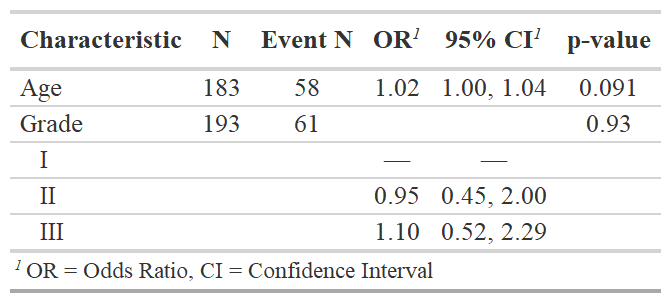
\includegraphics[scale=0.49]{uvregression.png}
  \centering
\end{figure}

\section{Inline Reporting}

Reproducible reports are an important part of good analysis practices.
We often need to report the results from a table in the text of an R markdown report.
The \code{inline\_text()}  function reports statistics from \pkg{gtsummary} tables inline in an R markdown document.

Imagine you need to report the results for age from the univariate table above.
Typically, the odds ratio, confidence interval, and p-value would be hard-coded into a report, which can lead to reproducibility issues if the data is updated and the hard-coded statistics are not amended.
A simple call to the \code{inline\_text()} function will dynamically add the model results to an RMarkdown report.

\begin{quote}
The odds ratio for age was \code{\textasciigrave{}r\ inline\_text(uvreg,\ variable\ =\ age)\textasciigrave{}}.
\end{quote}

Here's how the line will appear in your report.

\begin{quote}
The odds ratio for age was 1.02 (95\% CI 1.00, 1.04; p=0.091).
\end{quote}

The default pattern to display for a regression table is \code{"\{estimate\} (\{conf.level*100\}\% CI \{conf.low\}, \{conf.high\}; \{p.value\})"} (again using glue syntax), and can be modified with the \code{inline\_text(pattern=)} argument. 

\section{Merging and Stacking}

The \pkg{gtsummary} tables shown above are often ready for publication as they are; however, it is common that more complex tables need to be constructed. This can be achieved by merging or stacking \pkg{gtsummary} tables using the \code{tbl\_merge()} and \code{tbl\_stack()} functions.
For example in cancer research, we often report two model for predicting a tumor's response to treatment and risk of death.
These two models are often reported side-by-side, and it's simple to construct using \code{tbl\_merge()}.
First, build a table for each regression model using \code{tbl\_regression()}, then merge the two tables with \code{tbl\_merge()}.
Any number of \pkg{gtsummary} tables can be merged with this function.

\begin{example}
tbl1 <- 
  glm(response ~ age + grade, trial, family = binomial) %>%
  tbl_regression(exponentiate = TRUE)

tbl2 <-
  coxph(Surv(ttdeath, death) ~ age + grade, trial) %>%
  tbl_regression(exponentiate = TRUE) 

tbl_merge_1 <-
  tbl_merge(
    tbls = list(tbl1, tbl2),
    tab_spanner = c("**Tumor Response**", "**Time to Death**")
  )
\end{example}
\newpage

\begin{figure}[h!]
  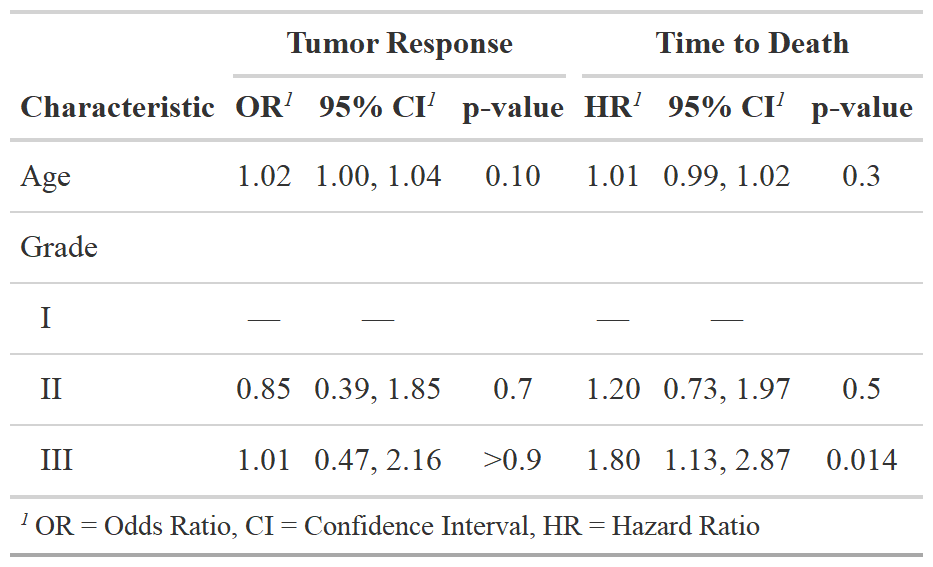
\includegraphics[scale=0.49]{merge.png}
  \centering
\end{figure}

Similarly, any number of \pkg{gtsummary} tables may be stacked using the \code{tbl\_stack()} function.

\section{Themes}

We love themes.
The default styling (e.g. statistics displayed in \code{tbl\_summary()}, how p-values are rounded, decimal separator, and more) follow the reporting guidelines from European Urology, The Journal of Urology, Urology, and the British Journal of Urology International \citep{assel2019guidelines}.
However, you'll likely submit to another journal, or your personal preferences differ from the defaults.
The \pkg{gtsummary} package is unique from other table building packages in the ability to set fine-grained customization defaults with themes. 
Themes were created to make these customizations easy to navigate and reuse across documents or projects. 
With themes, users can control default settings for existing functions (e.g. always present means instead of medians in \code{tbl\_summary()}), as well as other changes that are not modifiable with function arguments.
Several themes are available to follow various journals' reporting guidelines, reduce cell padding and font size, and recently language themes were introduced translating \pkg{gtsummary} tables to more than 10 languages.

For example, using the theme for New England Journal of Medicine, large p-values are rounded to two decimal places and confidence intervals are shown as \code{"lb to ub"} instead of \code{"lb, ub"} (among other modifications). 

% \newpage
\begin{example}
theme_gtsummary_journal("nejm")

glm(response ~ age + grade, trial, family = binomial) %>%
  tbl_regression(exponentiate = TRUE)
\end{example}

\begin{figure}[h!]
  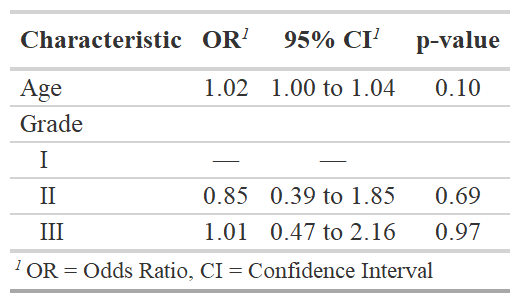
\includegraphics[scale=0.49]{nejm.png}
  \centering
\end{figure}

A custom theme was used to construct the \pkg{gtsummary} tables shown in this manuscript to match the \emph{R Journal} font and reduce the default cell padding. 
Themes are an evolving feature and we welcome additions of new journals' reporting guidelines or other themes useful to users.
A full glossary of customizable theme elements is available in the package's themes vignette (\url{http://www.danieldsjoberg.com/gtsummary/articles/themes.html}).

\section{Print Engines}

Tables printed with \pkg{gtsummary} can be seamlessly integrated into R markdown documents and knitted into various output types using a number of print engines.
The package was written to be a companion to the \pkg{gt} package from RStudio and is optimized to leverage the advanced customization features of this print engine, but offers compatibility with a variety of popular printing methods including \code{knitr::kable()} \citep{knitr}, \CRANpkg{flextable}  \citep{flextable}, \CRANpkg{huxtable} \citep{huxtable}, and \CRANpkg{kableExtra} \citep{kableExtra}.
While \pkg{gt} is used as default for most outputs, you can easily convert to using your print engine of choice using several conversion helper functions provided in the package (e.g. \code{as\_kable()}).
The package is designed to interact with these print engines behind the scenes to reduce burden on users, and you generally only need to be aware of them if you want to add advanced customizations.
The default print engine can be systematically set using \pkg{gtsummary} themes.

\section{Summary}

The functions in the \pkg{gtsummary} package were designed to reduce the burden of reporting, and to work together to easily construct both simple and complex tables.
It is our hope that the user-friendly syntax and publication-ready tables will aid analysts in preparing reproducible and high-quality findings.

\bibliography{RJreferences}

\address{Daniel D. Sjoberg\\
  Memorial Sloan Kettering Cancer Center\\
  1275 York Ave., New York, New York 10022\\
  USA\\
  ORCiD: 0000-0003-0862-2018\\
  \email{sjobergd@mskcc.org}}

\address{Karissa Whiting\\
  Memorial Sloan Kettering Cancer Center\\
  1275 York Ave., New York, New York 10022\\
  USA\\
  ORCiD: 0000-0002-4683-1868\\
  \email{whitingk@mskcc.org}}

\address{Michael Curry\\
  Memorial Sloan Kettering Cancer Center\\
  1275 York Ave., New York, New York 10022\\
  USA\\
  ORCiD: 0000-0002-0261-4044\\
  \email{currym1@mskcc.org}}
